%%%%%%%%%%%%%%%%%%%%%%%%%%%%%%%%%%%%%%%%%
% Beamer Presentation
% LaTeX Template
% Version 1.0 (10/11/12)
%
% This template has been downloaded from:
% http://www.LaTeXTemplates.com
%
% License:
% CC BY-NC-SA 3.0 (http://creativecommons.org/licenses/by-nc-sa/3.0/)
%
%%%%%%%%%%%%%%%%%%%%%%%%%%%%%%%%%%%%%%%%%

%----------------------------------------------------------------------------------------
%	PACKAGES AND THEMES
%----------------------------------------------------------------------------------------

\documentclass{beamer}

\newcommand{\EMSE}{ {\rm EMSE}}
\newcommand{\CC}{ {\rm CC}}
\newcommand{\MSE}{ {\rm MSE}}
\newcommand{\WIN}{\scriptscriptstyle {\rm WIE}}
\newcommand{\OROI}{\scriptscriptstyle {\rm out ROI}}
\newcommand{\Her}{\scriptscriptstyle H}
\newcommand{\T}{\scriptscriptstyle T}
\newcommand{\LMS}{\scriptscriptstyle {\rm LMS}}
\newcommand{\RDE}{\scriptscriptstyle {\rm RDE}}
\newcommand{\MRD}{\scriptscriptstyle {\rm MRD}}
\newcommand{\MSD}{\scriptscriptstyle {\rm MSD}}
\newcommand{\SBD}{\scriptscriptstyle {\rm SBD}}
\newcommand{\SDD}{\scriptscriptstyle {\rm SDD}}
\newcommand{\WIE}{\scriptscriptstyle {\rm WIE}}
\newcommand{\R}{\scriptscriptstyle {\rm R}}
\newcommand{\I}{\scriptscriptstyle {\rm I}}
\newcommand{\mT}{\scriptscriptstyle -T}
\newcommand{\vir}{,\hspace{-0.15ex}}
\newcommand{\M}{\scriptscriptstyle M}
\newcommand{\MMA}{\rm \scriptscriptstyle MMA}
\newcommand{\neigh}{\scriptscriptstyle {\rm neigh}}
\newcommand{\st}{\scriptscriptstyle {\rm st}}
\newcommand{\nd}{\scriptscriptstyle {\rm nd}}
\newcommand{\CSD}{\scriptscriptstyle {\rm CSD}}
\newcommand{\E}{{\rm E}}
\newcommand{\uM}{{\mathbf u}}
\newcommand{\rM}{{\mathbf r}}
\newcommand{\xM}{{\mathbf x}}
\newcommand{\yM}{{\mathbf y}}
\newcommand{\XM}{{\mathbf X}}
\newcommand{\w}{{\mathbf w}}
\newcommand{\wo}{{\mathbf{w}}_{\rm o}}
\newcommand{\q}{{\mathbf q}}
\newcommand{\qp}{{\mathbf {\dot{q}}}}
\newcommand{\Nuquad}{\|{\mathbf u(n)}\|^2}
\newcommand{\NuquadP}{\|{\mathbf u(n)}\|^2_{{\mathbf R}^{-1}(n)}}
\newcommand{\uMc}{{\mathbf u}^{\ast}}
\newcommand{\wtil}{\widetilde{\mathbf w}}
\newcommand{\Dw}{\boldsymbol{\Delta}{\mathbf w}}
\newcommand{\Dewp}{\boldsymbol{\Delta}{\mathbf{\dot{w}}}}
\newcommand{\Pb}{{\mathbf R}^{-1}}
\newcommand{\ebari}{{\bar{e}}_i}
\newcommand{\field}[1]{\mathbb{#1}}
\newcommand{\re}{\field{R}}
\newcommand{\co}{\field{C}}
\newcommand{\CO}{\field{C}}
\newcommand{\RE}{\field{R}}
\newcommand{\Tr}{{\rm Tr}}
\newcommand{\Ru}{{\mathbf R}}
\newcommand{\sgbeta}{\sigma_{\scriptscriptstyle{\!\alpha}}^2}
\newcommand{\sgphi}{\sigma_{\scriptscriptstyle{\!\varphi}}^2}
\newcommand{\cred}{\textcolor{red}}
\newcommand{\lbo}{\lambda_{\rm o}}
\newcommand{\cond}{\mathbf{w}_1(n\!-\!1),\mathbf{w}_{2}(n\!-\!1)}
\newcommand{\cb}{\textcolor{blue}}
\newcommand{\pu}{\mathbf{p}_{\!\scriptscriptstyle \Delta}}
\definecolor{laranja}{rgb}{0.8,0.5,0}
\newcommand{\crt}{\textcolor{laranja}}
\newcommand{\Psibf}{\boldsymbol{\Psi}}
\newcommand{\Sigmabf}{\boldsymbol{\Sigma}}
\newcommand{\epsbf}{\boldsymbol{\epsilon}}
\newcommand{\betabf}{\boldsymbol{\beta}}
\newcommand{\alphabf}{\boldsymbol{\alpha}}
\newcommand{\thetabf}{\boldsymbol{\theta}}
\newcommand{\gammabf}{\boldsymbol{\gamma}}
\newcommand{\lambdabf}{\boldsymbol{\lambda}}
\newcommand{\ML}{{\rm ML}}
\newcommand{\LS}{{\rm LS}}
\newcommand{\SSS}{{\rm SS}}
\newcommand{\UPS}{{\rm UPS}}
\newcommand{\PS}{{\rm PS}}

\mode<presentation> {

% The Beamer class comes with a number of default slide themes
% which change the colors and layouts of slides. Below this is a list
% of all the themes, uncomment each in turn to see what they look like.

%\usetheme{default}
%\usetheme{AnnArbor}
%\usetheme{Antibes}
%\usetheme{Bergen}
%\usetheme{Berkeley}
%\usetheme{Berlin}
%\usetheme{Boadilla}
\usetheme{CambridgeUS}
%\usetheme{Copenhagen}
%\usetheme{Darmstadt}
%\usetheme{Dresden}
%\usetheme{Frankfurt}
%\usetheme{Goettingen}
%\usetheme{Hannover}
%\usetheme{Ilmenau}
%\usetheme{JuanLesPins}
%\usetheme{Luebeck}
%\usetheme{Madrid}
%\usetheme{Malmoe}
%\usetheme{Marburg}
%\usetheme{Montpellier}
%\usetheme{PaloAlto}
%\usetheme{Pittsburgh}
%\usetheme{Rochester}
%\usetheme{Singapore}
%\usetheme{Szeged}
%\usetheme{Warsaw}

% As well as themes, the Beamer class has a number of color themes
% for any slide theme. Uncomment each of these in turn to see how it
% changes the colors of your current slide theme.

%\usecolortheme{albatross}
%\usecolortheme{beaver}
%\usecolortheme{beetle}
%\usecolortheme{crane}
%\usecolortheme{dolphin}
%\usecolortheme{dove}
%\usecolortheme{fly}
%\usecolortheme{lily}
%\usecolortheme{orchid}
%\usecolortheme{rose}
%\usecolortheme{seagull}
%\usecolortheme{seahorse}
%\usecolortheme{whale}
%\usecolortheme{wolverine}

%\setbeamertemplate{footline} % To remove the footer line in all slides uncomment this line
\setbeamertemplate{footline}[page number] % To replace the footer line in all slides with a simple slide count uncomment this line

\setbeamertemplate{navigation symbols}{} % To remove the navigation symbols from the bottom of all slides uncomment this line
}

\usepackage{graphicx} % Allows including images
\usepackage{booktabs} % Allows the use of \toprule, \midrule and \bottomrule in tables
\usepackage{color}
\usepackage{amsmath}

%----------------------------------------------------------------------------------------
%	TITLE PAGE
%----------------------------------------------------------------------------------------

\title[TopicModel]{Topic Modeling of Document collections} % The short title appears at the bottom of every slide, the full title is only on the title page

\author{Jer\'onimo Arenas-Garc\'{\i}a, Vanessa G\'omez-Verdejo, Jes\'us Cid-Sueiro} % Your name
\institute[UC3M] % Your institution as it will appear on the bottom of every slide, may be shorthand to save space
{
Universidad Carlos III de Madrid \\ % Your institution for the title page
\medskip
\textit{jeronimo.arenas@uc3m.es} % Your email address
}
\date{March 24, 2021}
%\date{\today} % Date, can be changed to a custom date

\begin{document}

%######################################################
%######################################################
\begin{frame}
\titlepage % Print the title page as the first slide
\end{frame}


%######################################################
%######################################################
\begin{frame}

    \frametitle{Contents}

	\large

    \begin{enumerate}
  
    	\item {\bf \color{blue}{Introduction}}
    	\item Latent Semantic Indexing
    	\item Latent Dirichlet Allocation
    	\item Gensim Overview
    
    \end{enumerate}

\end{frame}

%######################################################
%######################################################
\section{1. Introduction}
\subsection{Introduction}

%######################################################
%######################################################
\begin{frame}

    \frametitle{Topic models}

	\large

    \begin{itemize}
  
    	\item Topic Models attempt to uncover the underlying semantic structure of a document corpus by identifying recurring patterns of terms (topics).
    	\vspace{1cm}
    	\item Topic models are models for bags-of-words:
    	\begin{itemize}
			\item do not parse sentences
			\item do not care about word order, and
			\item do not ``understand'' grammar or syntax
		\end{itemize}

    
    \end{itemize}

\end{frame}

%######################################################
%######################################################
\begin{frame}

    \frametitle{Topic models}

	\footnotesize

    \begin{itemize}
  
		\item Topic models are useful on their own to build visualizations and explore data. They are also very useful as an intermediate step in many other tasks.
		
        \begin{columns}
        \begin{column}{0.48\textwidth}
        \begin{exampleblock}{1. Identification and characterization of the main topics of a Document Collection}
           \centerline{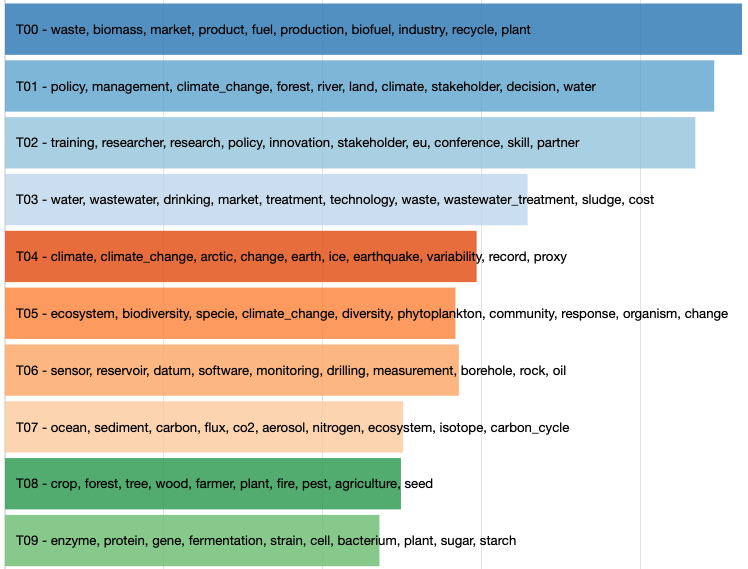
\includegraphics[width=\textwidth]{./figs/topics.png}}
        \end{exampleblock}
        \end{column}
        \begin{column}{0.48\textwidth}  %%<--- here
        \begin{exampleblock}{2. Obtaining a (semantic) vector representation of each document in the collection(s)}
           \centerline{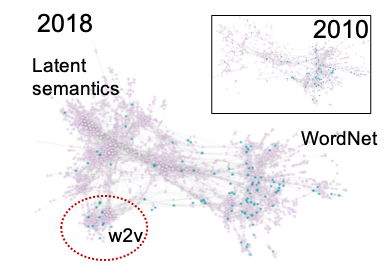
\includegraphics[width=\textwidth]{./figs/graph.png}}
        \end{exampleblock}
        \end{column}
        \end{columns}

    \end{itemize}

\end{frame}


%######################################################
%######################################################
\begin{frame}

    \frametitle{Topic modeling tools}

	\begin{itemize}
  
    	\item {\bf Gensim} is an NLP toolbox Developed by Radim Rehurek, and specialized in topic modeling and semantic analysis of texts. It includes:
    	\begin{itemize}
			\item Tools for BoW codification of documents
			\item Tools for TF-IDF representation of documents
			\item {\color{blue}{\bf Latent Semantic Indexing (LSA/LSI)}}
			\item {\color{blue}{\bf Latent Dirichlet Allocation (LDA)}}
			\item Dynamic topic modeling (incomplete)
			\item Word2Vec tools for mapping words in a vector semantic space
		\end{itemize}
		\item In the block we will rely on David Blei's LDA algorithm that rely on the BoW representations. Other available Python implementations are:
		\begin{itemize}
			\item LDA toolbox
			\item Scikit learn implementation
			\item GraphLab (based on collapsed Gibbs sampling)
		\end{itemize} 
		\item {\color{blue}{\bf MALLET}} contains a well-known Java implementation of LDA
    
    \end{itemize}

\end{frame}

%######################################################
%######################################################
\begin{frame}

    \frametitle{Topic model visualizers}

	Given the extended use of topic models, some researchers have also publish tools for visualizing the results of topic models.

    \begin{itemize}
  
    	\item dfr-browser: \url{https://github.com/agoldst/dfr-browser} \\
    	Demo: \url{https://agoldst.github.io/dfr-browser/demo/}
    	
    	\item {\color{blue}{\bf pyLDAvis:}} \url{https://github.com/bmabey/pyLDAvis} \\
    	
    	\item Topic model visualization Engine (TMVE): \url{https://github.com/ajbc/tmve-original} \\
    	Demo: \url{http://www.princeton.edu/~achaney/tmve/wiki100k/browse/topic-presence.html} 
    
    \end{itemize}

\end{frame}


%######################################################
%######################################################
\begin{frame}

    \frametitle{Contents}

	\large

    \begin{enumerate}
  
    	\item Introduction
    	\item {\bf \color{blue}{Latent Semantic Indexing}}
    	\item Latent Dirichlet Allocation
    	\item Gensim Overview
    
    \end{enumerate}

\end{frame}

%######################################################
%######################################################
\section{2. Latent Semantic Indexing}
\subsection{LSI}

%######################################################
%######################################################
\begin{frame}
    \frametitle{Latent Semantic Indexing}
    
    \begin{itemize}
    \item It transforms documents from either
        \begin{itemize}
            \item bag-of-words, or
            \item (preferably) TFIDF document representation
        \end{itemize}
        into a latent space of a lower dimensionality (number of topics)
    \vspace{.2cm}
    \item LSI is able to identify correlations among semantically related terms that are latent in a collection of text documents
    \vspace{.2cm}
    \item When used to measure similarity among documents, LSI overcomes two of the most problematic constraints of Boolean keyword queries: synonyms and polysemy.
    \end{itemize}
\end{frame}


%######################################################
%######################################################
\begin{frame}
\frametitle{Latent Semantic Indexing}
    
    The starting point of LSI is the TF-IDF matrix, $\mathbf A$, with size $(d \times t)$,
    \begin{itemize}
        \item $d$ is the number of documents
        \item $t$ is the number of terms in the vocabulary
    \end{itemize}
    
    \vspace{1cm}
    
    \begin{columns}
        \begin{column}{0.3\textwidth}
        \centerline{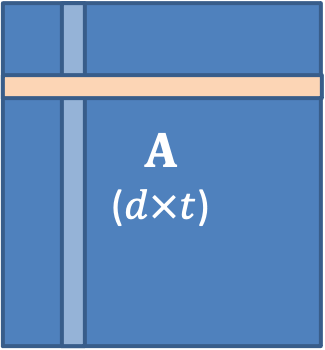
\includegraphics[width=.7\textwidth]{./figs/TFIDF_matrix.png}}
        \end{column}
        \begin{column}{0.5\textwidth}  %%<--- here
        \begin{itemize}
            \item $i$th row: TFIDF representation of document $i$
            \item $i$th column: associated to term $i$ in the vocabulary
        \end{itemize}
        \end{column}
    \end{columns}
    
    
    
\end{frame}

%######################################################
%######################################################
\begin{frame}
\frametitle{Latent Semantic Indexing}
\footnotesize
LSI computes the term and document vector spaces by means of the singular value decomposition (SVD) of matrix $\mathbf A$, with rank $r$, into the product of 3 matrices:
$${\mathbf A} = {\mathbf D} {\mathbf S} {\mathbf T}^\top$$

\begin{itemize}
    \item ${\mathbf D} (d\times r)$: Unitary document-concept matrix (${\mathbf D}^\top {\mathbf D} = {\mathbf I}_r$) 
    \item ${\mathbf T} (t\times r)$: Unitary term-concept matrix (${\mathbf T}^\top {\mathbf T} = {\mathbf I}_r$) 
    \item ${\mathbf S} (r\times r)$: Diagonal matrix of singular values
    $$(s_0>s_1>\dots>s_{r-1}>0)$$
\end{itemize}
\centerline{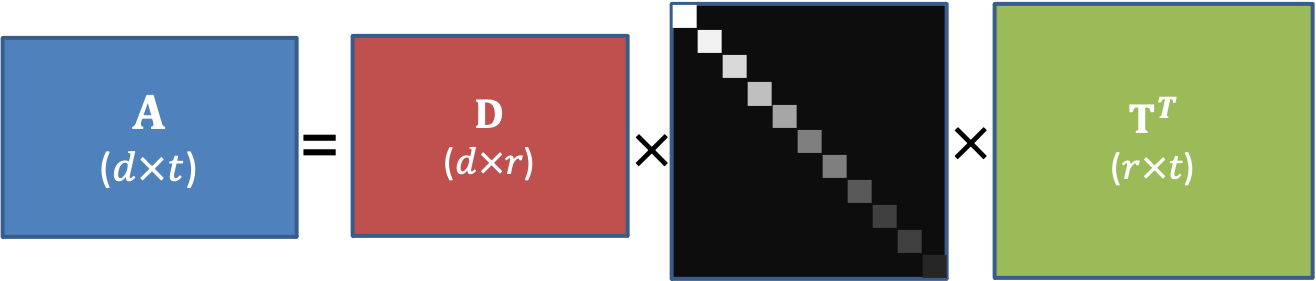
\includegraphics[width=\textwidth]{./figs/SVD.png}}

(Note that elements in ${\mathbf D}$ and ${\mathbf T}$ can have any sign.)
    
\end{frame}



%######################################################
%######################################################
\begin{frame}
\frametitle{Latent Semantic Indexing}
LSI approximates $\mathbf A$ using a reduced number $k$ of concepts (the topics in LSI), by ignoring the smallest values.
$${\mathbf A} \approx {\mathbf D}_k {\mathbf S}_k {\mathbf T}_k^\top$$

\centerline{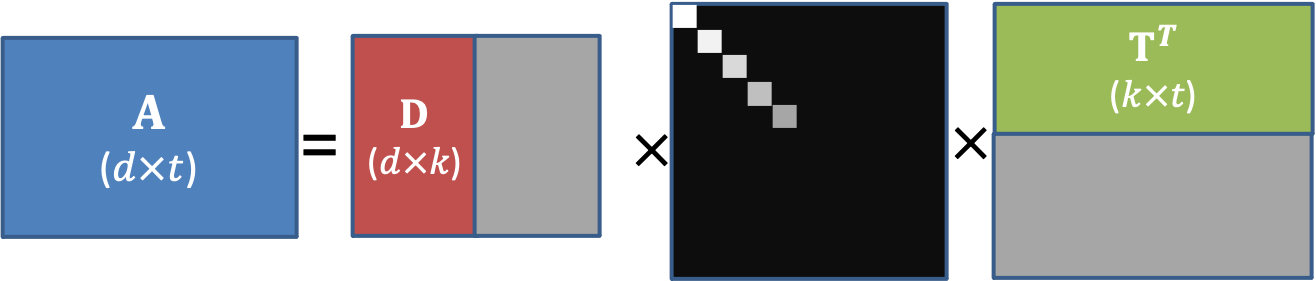
\includegraphics[width=.8\textwidth]{./figs/SVD_k.png}}

\vspace{.5cm}

\centerline{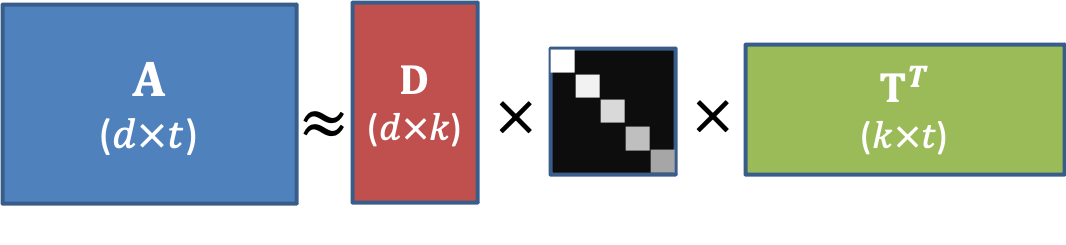
\includegraphics[width=.6\textwidth]{./figs/SVD_k2.png}}

\end{frame}




%######################################################
%######################################################
\begin{frame}
    \frametitle{Latent Semantic Indexing}
    
Note that the $n$th row of ${\mathbf A}$ depends only on the $n$th row of ${\mathbf D}$

\begin{itemize}
    \item The $n$th row of ${\mathbf D}$ is the ``latent'' representation of the $n$th document
    \item The TFIDF representation of the $n$th document is approximated a linear combination of columns in ${\mathbf T}$ (rows of ${\mathbf T}^\top$)
    \item Each column of ${\mathbf T}$ (of size $t \times 1$) is the characterization of a different LSI ``topics''
\end{itemize}

\centerline{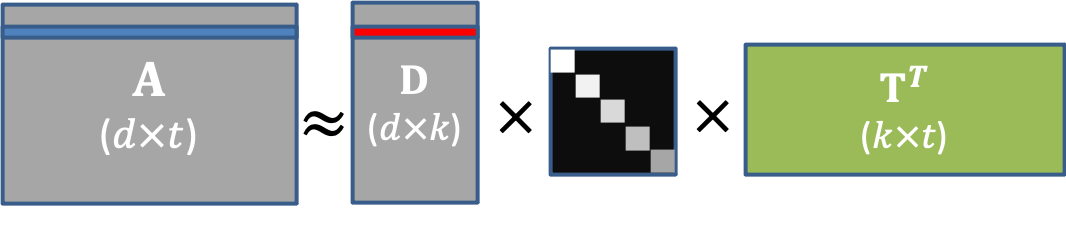
\includegraphics[width=.8\textwidth]{./figs/SVD_k3.png}}

\begin{block}{Intuitive explanation}
Since the SVD provides the best reduced-rank approximation of $\mathbf A$, this implies that the topic matrix will be adjusted accordingly, aligning the topic vectors with the dominant themes in the corpus.
\end{block}

\end{frame}


%######################################################
%######################################################
\begin{frame}

    \frametitle{Contents}

	\large

    \begin{enumerate}
  
    	\item Introduction
    	\item Latent Semantic Indexing
    	\item {\bf \color{blue}{Latent Dirichlet Allocation}}
    	\item Gensim Overview
    
    \end{enumerate}

\end{frame}

%######################################################
%######################################################
\section{3. Latent Dirichelet Allocation}
\subsection{LDA}


%######################################################
%######################################################
\begin{frame}

    \frametitle{Latent Dirichlet Allocation}

	\begin{itemize}
	    \item LDA is another transformation from bag-of-words into a latent topic space of lower dimensionality
	    \vspace{.3cm}
	   \item LDA is a probabilistic extension of LSI. It assumes a generative model where
	    \begin{itemize}
	        \item topics are characterized by probability distributions over words
	        \item documents are characterized by probability distributions over topics
	    \end{itemize}
	   \vspace{.3cm}
	   \item These distributions are inferred automatically from a training corpus
	\end{itemize}

\end{frame}


%######################################################
%######################################################
\begin{frame}

    \frametitle{Latent Dirichlet Allocation}

	\centerline{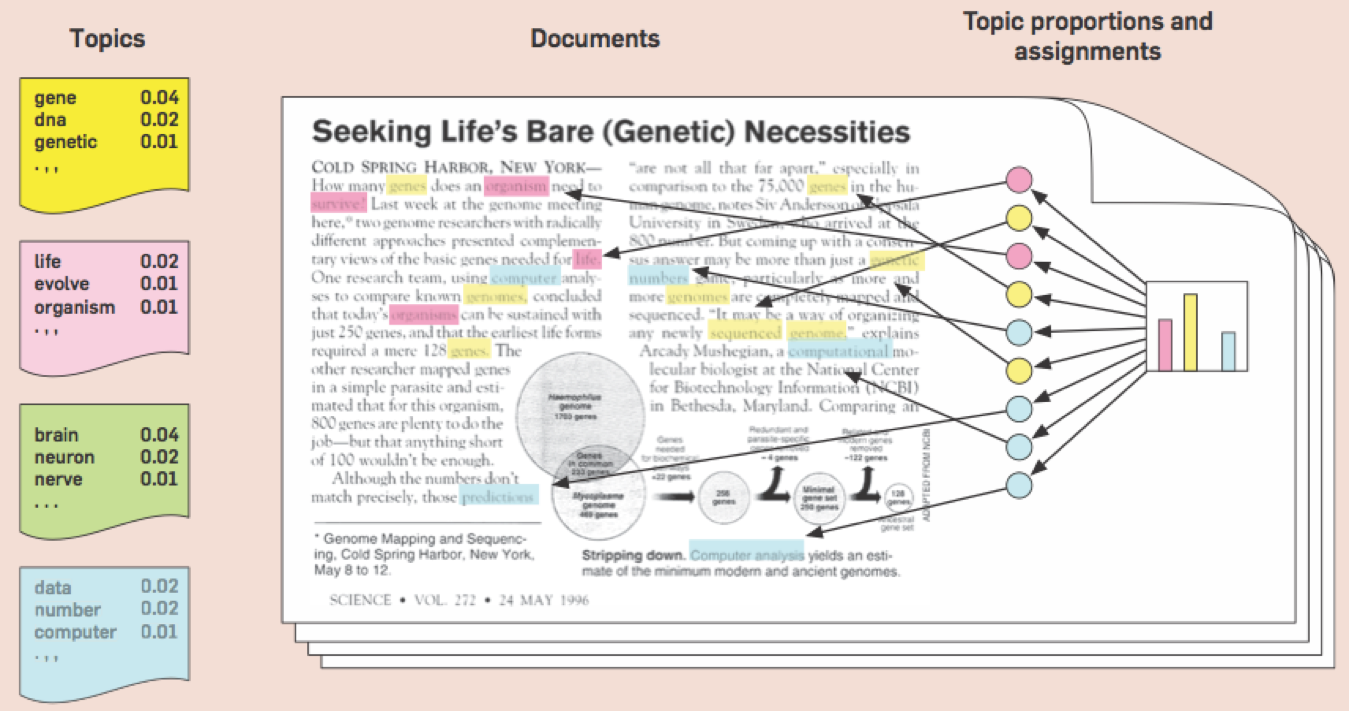
\includegraphics[width=\textwidth]{./figs/NLPTM_LDA.png}}
\tiny	
(Image taken from \url{http://www.cs.columbia.edu/~blei/papers/Blei2012.pdf})

\end{frame}

%######################################################
%######################################################
\begin{frame}

    \frametitle{Maximum Likelihood and Maximum a Posteriori Estimation}
    
    \begin{enumerate}
        \item Propose a parameterized generative model
        \item For the available observations, write down the likelihood function, i.e., the joint probability of observations for a given set of parameter values
        \item Find the parameter values that maximize the likelihood function
        
    \end{enumerate}

	\centerline{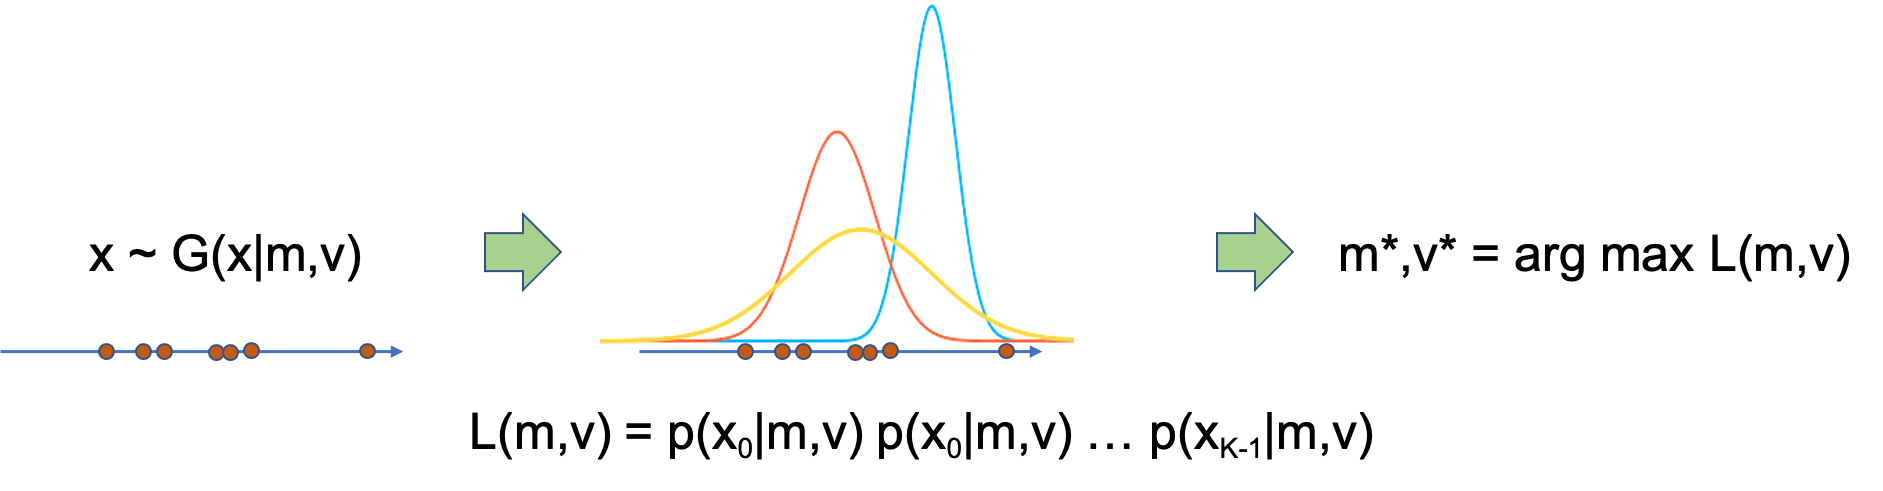
\includegraphics[width=\textwidth]{./figs/ML_Gauss.png}}
	
	In maximum {\em a posteriori}, we assume some {\em prior} distribution for the unknown parameters, and maximize their {\em a posteriori} distribution, taking into account that:
	$$posterior \propto (likelihood \times prior)$$

\end{frame}



%######################################################
%######################################################
\begin{frame}


    \frametitle{Understanding LDA}

	LDA is also based on MAP estimation of the parameters of a generative probabilistic model for document production: 
	\begin{itemize}
	\item Documents have been generated according to some probability model with some unknown parameters and certain hidden variables
	\item Our observations are the documents
	\item The corpus data is used to infer the topic structure (hidden variables) from the words of documents (observed variables)
	\centerline{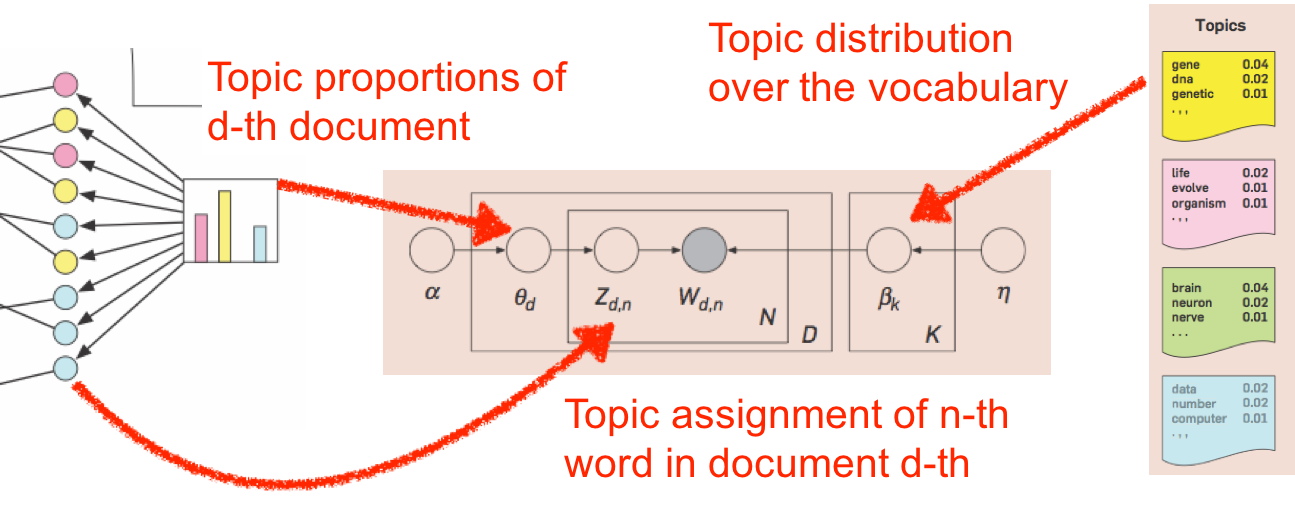
\includegraphics[width=.7\textwidth]{./figs/NLPTM_LDA2.png}}
	\end{itemize}

\end{frame}


%######################################################
%######################################################
\begin{frame}

    \frametitle{The Dirichlet Distribution}
    
    The Dirichlet distribution is frequently used to generate probability vectors. For instance, when we sample a 3D Dirichlet distribution, we will obtain triplets of positive numbers that sum up to 1.

	\centerline{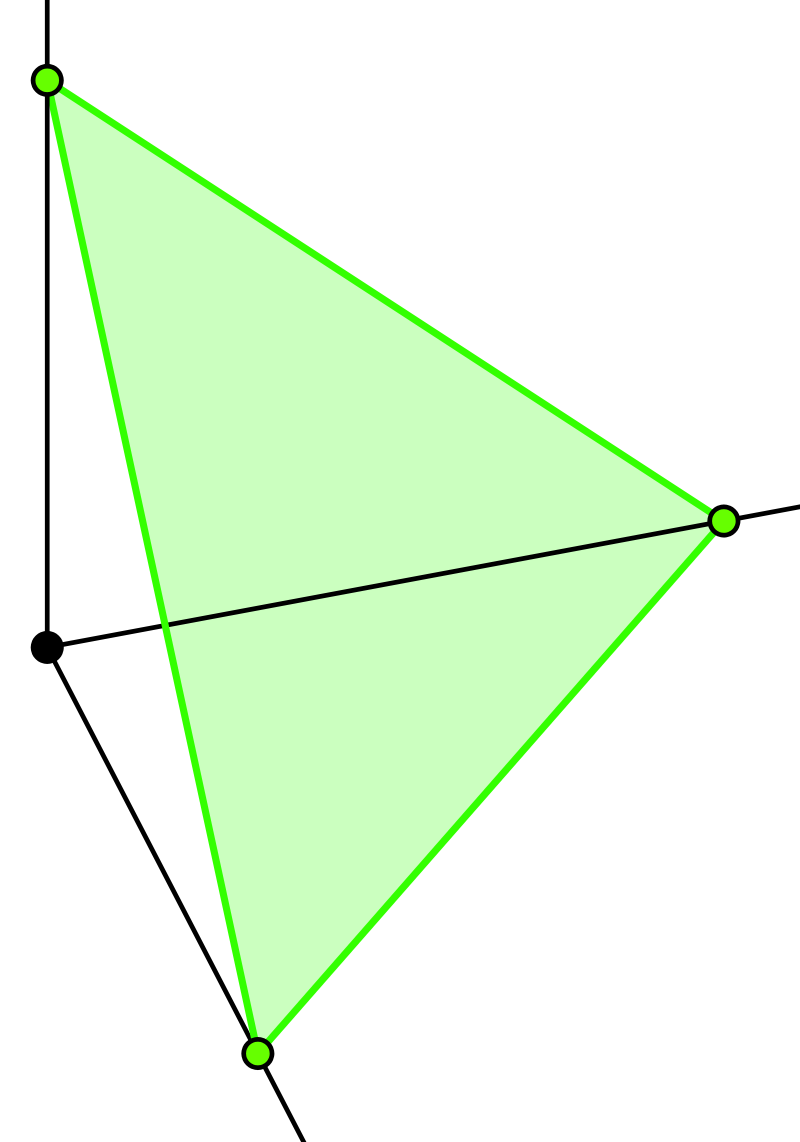
\includegraphics[width=.25\textwidth]{./figs/simplex.png}~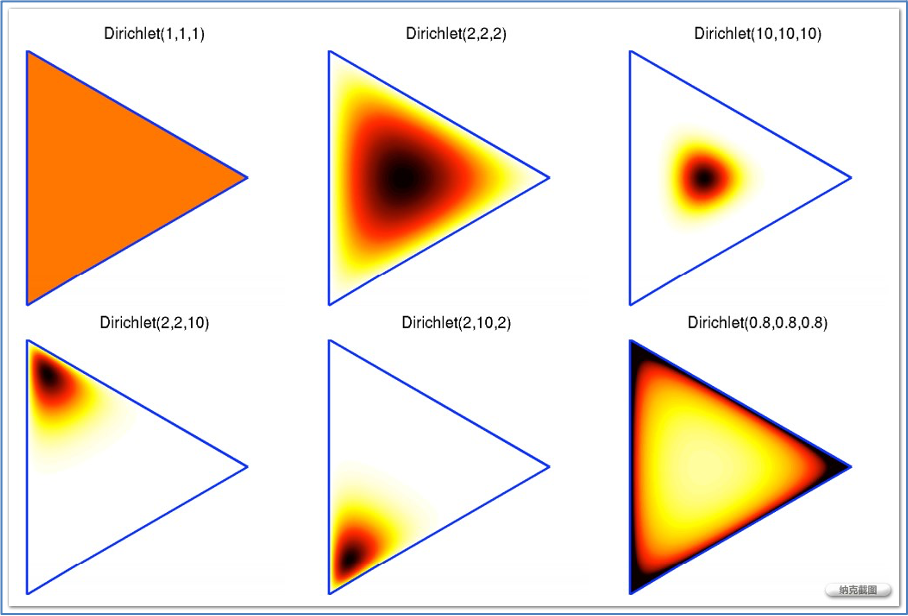
\includegraphics[width=.6\textwidth]{./figs/dirichlet.png}}
	\tiny
	Image taken from http://www.cnblogs.com/huashiyiqike/articles/3232082.html

\end{frame}


%######################################################
%######################################################
\begin{frame}

    \frametitle{LDA generative model}

	\centerline{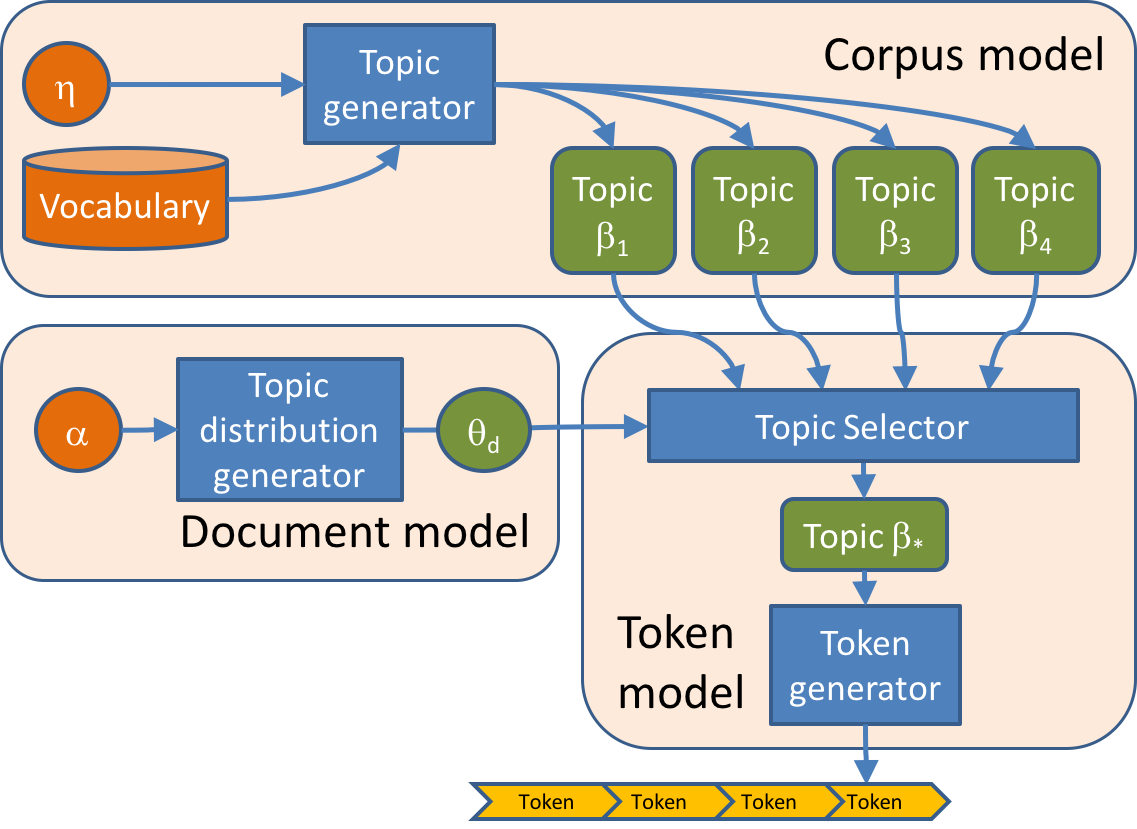
\includegraphics[width=.9\textwidth]{./figs/NLPTM_LDA3.png}}

\end{frame}

%######################################################
%######################################################
\begin{frame}

    \frametitle{LDA generative model (II)}
    
    \footnotesize

	\begin{block}{Topic generator}
	\begin{itemize}
	\item Generates tokens distributions by means of a Dirichlet distribution with concentration parameter $\eta$.
	\item Each topic is therefore characterized by a vector $\boldsymbol{\beta}_t$ that indicates the term distribution for the given topic
	\item Small $\eta$ implies that topic distributions will be concentrated in a few distinct tokens (only a few non-zero components in each $\boldsymbol{\beta}_t$).
	\end{itemize}
	\end{block}
	\begin{block}{Document generator}
	\begin{itemize}
	\item For each document, generate its topic distribution by sampling a Dirichlet distribution with concentration parameter $\alpha$.
	\item Small $\alpha$ implies that for most documents only a few topics will be relevant.
	\item For each word in the document:
	\begin{enumerate}
	\footnotesize
		\item Select a topic according to a multinomial distribution with parameters given by the topic distribution for the document
		\item Select a word according to a multinomial distribution with parameters given by the word distribution for the selected topic
	\end{enumerate}

	\end{itemize}

	\end{block}

\end{frame}

%######################################################
%######################################################
\begin{frame}

    \frametitle{LDA optimization}

	\small
	\begin{itemize}
	\item The generative process for LDA corresponds to the following joint distribution of the hidden and observed variables
	\footnotesize
	$$p({\boldsymbol{\beta}}_{1:K}, {\boldsymbol{\theta}}_{1:D}, {\bf z}_{1:D}, w_{1:D}) = \prod_{i=1}^K p({\boldsymbol{\beta}}_i) \prod_{d=1}^D p({\boldsymbol{\theta}}_d) \left( \prod_{n=1}^{N_d} p({z}_{d,n}|{\boldsymbol{\theta}}_d) p({w}_{d,n} | {z}_{d,n}, {\boldsymbol{\beta}}_{1:K}) \right)$$
	

	\small
	\item Goal: computing the conditional distribution of the topic structure given the observed documents
	\footnotesize
	$$p({\boldsymbol{\beta}}_{1:K}, {\boldsymbol{\theta}}_{1:D}, {\bf z}_{1:D} | w_{1:D}) = \frac{p({\boldsymbol{\beta}}_{1:K}, {\boldsymbol{\theta}}_{1:D}, {\bf z}_{1:D}, w_{1:D})}{p(w_{1:D})}$$
	\small
	\item The denominator is the probability of seeing the observed corpus under any topic model. It can be computed by summing the joint distribution over every possible hidden topic structure, so its computation is not feasible.
	\item LDA implementations are based on:
	\begin{itemize}
	\item Variational Bayes implementations
	\item Sampling-based algorithms (typically, collapsed Gibbs-sampling with the goal of estimating word-assignments, ${\bf z}_{1:D}$)
	\end{itemize}
	
	\end{itemize}

\end{frame}

%######################################################
%######################################################
\begin{frame}

    \frametitle{LDA optimization (II)}

	After optimization, we will be mostly interested on the outcome of the Dirichlet distributions:
	\vspace{.5cm}
	\begin{itemize}
	\item ${\boldsymbol{\theta}}_{1:D}$ provide the topic representation for each document in the collection.
	\item ${\boldsymbol{\beta}}_{1:K}$ provide the probability distribution over the vocabulary of each identified topic.
	\item We will ignore the estimated assignments of each word ($z_{d,n}$)

	\end{itemize}
	
	\vspace{1cm}
	
	The average of the topic representation of all documents (${\boldsymbol{\theta}}_{1:D}$) is an estimation of the relative size of topics in the corpus.

\end{frame}



%######################################################
%######################################################
\subsection{Topic visualization}

%######################################################
%######################################################
\begin{frame}

    \frametitle{Topic visualization using pyLDAvis}

	\centerline{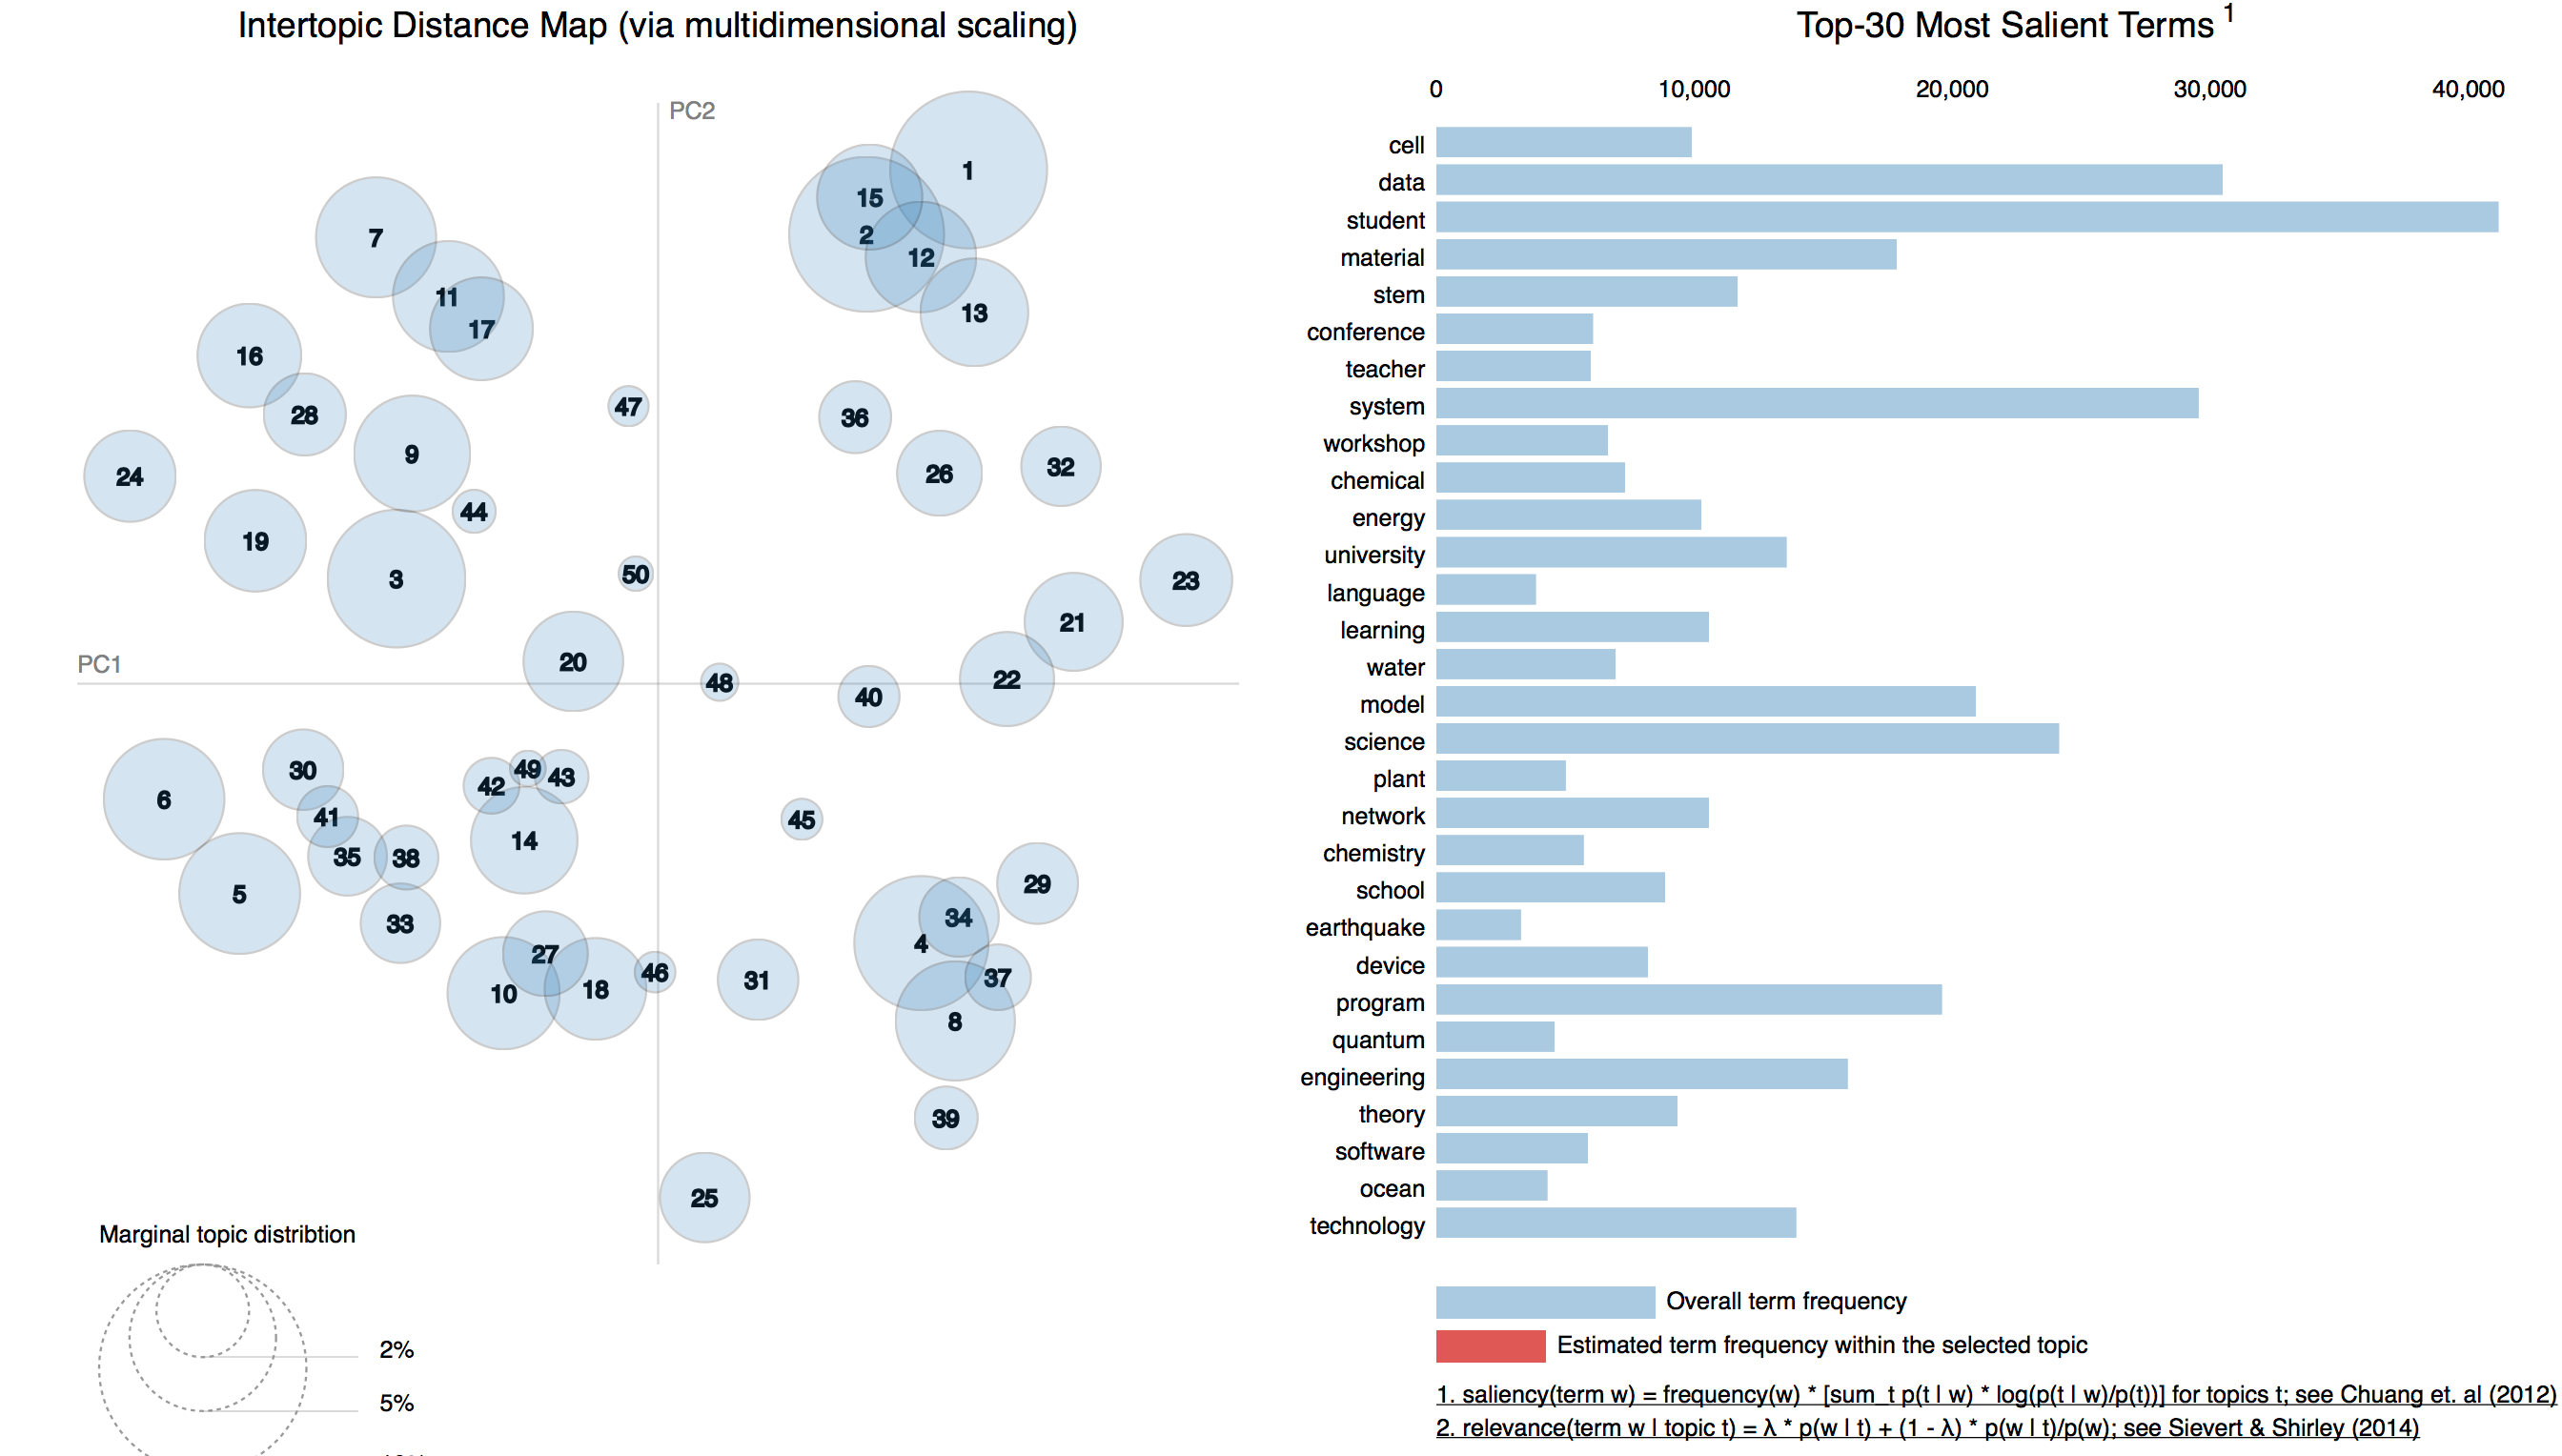
\includegraphics[width=\textwidth]{./figs/NLPTM_pyLDAvis.png}}
	
\end{frame}



%######################################################
%######################################################
\begin{frame}

    \frametitle{Contents}

	\large

    \begin{enumerate}
  
    	\item Introduction
    	\item Latent Semantic Indexing
    	\item Latent Dirichlet Allocation
    	\item {\bf \color{blue}{Gensim Overview}}
    
    \end{enumerate}

\end{frame}

%######################################################
%######################################################
\section{4. Gensim}
\subsection{Gensim}


%######################################################
%######################################################
\begin{frame}[fragile]

    \frametitle{Document BoW and TFIDF representation}

\begin{verbatim}
from gensim import corpora
from gensim import models

D = corpora.Dictionary(docs)
corpus_bow = [D.doc2bow(doc) for doc in docs]

tfidf = models.TfidfModel(corpus_bow)
corpus_tfidf = tfidf[corpus_bow]


    
\end{verbatim}

\end{frame}


%######################################################
%######################################################
\begin{frame}[fragile]

    \frametitle{Latent Semantic Indexing}

\begin{verbatim}
# Initialize an LSI transformation. 
# On real corpora, target dimensionality of
# 200-500 is a resonable first guess

lsi = models.LsiModel(corpus_tfidf,
    id2word=D, num_topics=200)

corpus_lsi = lsi[corpus_tfidf]

#It allows incremental updates
lsi.add_documents(another_tfidf_corpus)
corpus_lsi = lsi[corpus_tfidf]
    
\end{verbatim}

\end{frame}

%######################################################
%######################################################
\begin{frame}[fragile]

    \frametitle{Latent Semantic Indexing (II)}

\begin{verbatim}
# Analyzing the topics

lsi.print_topics(2)

topic #0(1.594): -0.703*"trees" + -0.538*"graph" + 
                 -0.402*"minors" +...
topic #1(1.476): -0.460*"system" + -0.373*"user" + 
                 -0.332*"eps" +....

# Analyzing document representation

print(corpus_lsi[0])

# "The intersection graph of paths in trees" 
[(0, -0.877), (1, -0.168)]

\end{verbatim}

\end{frame}

%######################################################
%######################################################
\begin{frame}[fragile]

    \frametitle{Latent Dirichlet Allocation}

\begin{verbatim}
# Create an LDA transformation
lda = models.LdaModel(corpus_bow,
    id2word=D, alpha='auto', num_topics=20)
    
# Analize topics
lda.print_topics(topics=2, topn=5)

# get topic probability distribution for a document
print(lda[doc_bow])

\end{verbatim}

\end{frame}


%######################################################
%######################################################
\begin{frame}

    \frametitle{Easter Assignments}

	\begin{enumerate}
  
    	\item Select and acquire a corpus of your own (default selection: ACL)
    	\item Homework to be published: Notebook on Sentiment Analysis using SpaCy
    	\item Review this presentation before next session
    \end{enumerate}

\end{frame}




\end{document} 